\section{REFERENCIAL TEÓRICO}	

\subsection{O BIODIESEL}
\hspace*{0.8cm}Biodiesel é uma denominação abrangente de combustíveis e aditivos provenientes de fontes renováveis. Um combustível que pode ser utilizado em substituição ao diesel comum, sem proporcionar danos mecânicos ao equipamento, além de possuir desempenho de igual qualidade em relação à potência, rendimento, etc. (BUMBA E YAMAMURA, 2015).

\begin{figure}[!htb]
\begin{center}
			\caption{Principais matérias primas para produção de biodiesel}
			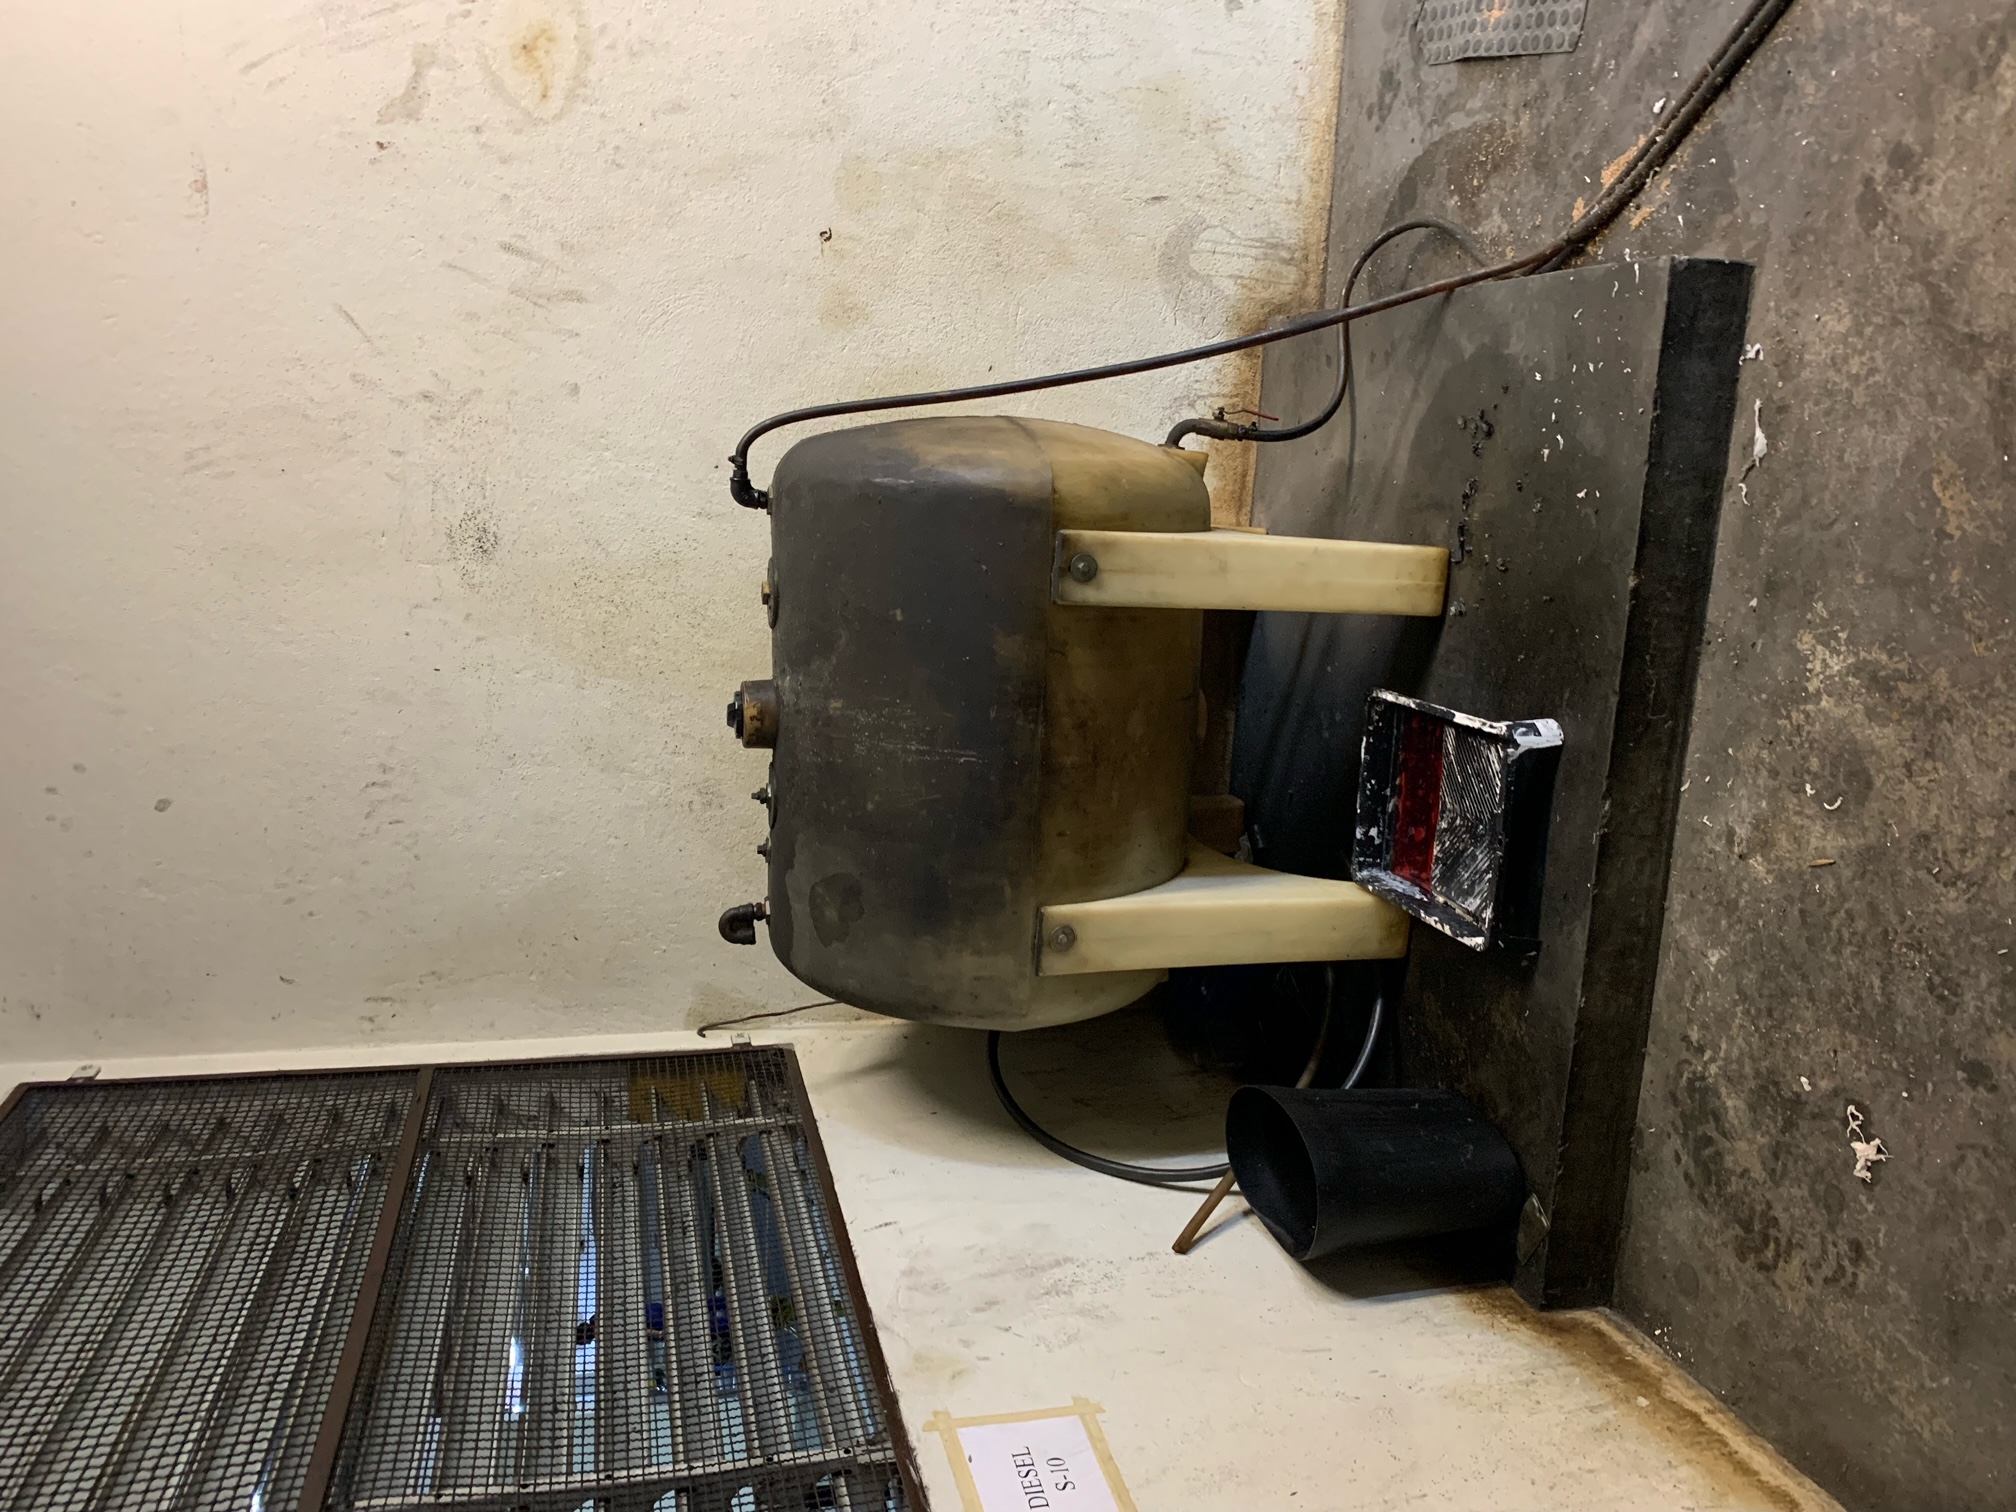
\includegraphics[width=.9\textwidth]{Figuras/image0.jpeg}
            \vspace*{\fill} 
            \begin{quote} 
            \centering 
            Fonte: Própria.
            \end{quote}
            \vspace*{\fill}
			\label{fig:ramcor}
\end{center}
\end{figure}

    O biodiesel pode ser produzido a partir de várias matérias-primas diferentes. É possível obter o combustível partindo de óleos vegetais, gorduras animais ou produtos residuais, como o óleo de fritura já usado. \cite{biodieselbr}.
    
    Importante ressaltar que o biodiesel não é só um produto nascido da necessidade de adaptações ou reciclagem. É um combustível de qualidade que pode ser utilizado em qualquer motor a diesel, com pouca ou nenhuma necessidade de adaptação, por vezes demonstrando desempenho até superior ao combustível padrão (DIAS, 2007).
    
\subsubsection{Impactos ambientais da substituição do Diesel mineral pelo Biodiesel}
    
\subsubsection{Utilização de Biodiesel em grupos geradores a Diesel}

\hspace{0.8cm}Assim como o diesel mineral, o biodiesel opera em motores de combustão-ignição. Pode ser usado como um substituto, mistura ou aditivo ao óleo diesel. Misturas de até 20\% de biodiesel (a 80\% de diesel convencional) podem ser usadas em praticamente qualquer equipamento diesel e são compatíveis com a maioria dos equipamentos de armazenamento e distribuição. Tais misturas (20\% ou menos) não requerem nenhuma modificação de motor e podem proporcionar performances próximas às do diesel. Misturas mais elevadas, ou até o biodiesel puro (100\% biodiesel, ou B100), podem ser usadas em muitos motores com pequenas alterações, posto que as propriedades físicas do Biodiesel são muito semelhantes às do Diesel. \cite{udaeta}

\subsubsection{O BIODIESEL A PARTIR DE ÓLEOS RESIDUAIS DE FRITURAS}

\hspace*{0.8cm}Atualmente, como não há uma legislação específica para o descarte de óleos residuais, muitos estabelecimentos descartam o óleo de fritura de forma inadequada, como por exemplo na rede de esgoto. Tal forma de descarte, resulta no entupimento de tubulações e consequente utilização de produtos químicos para desentupir as tubulações, produtos estes que são tóxicos e ocasionam danos ambientais juntamente com o óleo. \cite{bumba}.

    Sabe-se que um litro de óleo pode contaminar 1 milhão de litros de água, quantidade esta suficiente para o consumo de uma pessoa durante 14 anos. Uma vez presente no meio ambiente de forma inadequada, o óleo, de menor densidade que a água,  permanece  na  superfície, criando uma barreira que dificulta a entrada de luz e a oxigenação, comprometendo assim a base da cadeia alimentar aquática. \cite{bilck}.
    
    Além da contaminação das águas, o óleo que atinge o leito de rios o impermeabiliza, favorecendo enchentes. \cite{felizardo}.

    Há três vantagens principais de se utilizar óleos residuais de frituras como matéria prima para a produção de biodiesel: a) no âmbito tecnológico, com a não necessidade do processo de extração do óleo; b) no âmbito econômico, devido à diminuição do custo da matéria prima com o resíduo de fritura; c) no âmbito ambiental, pois destina-se adequadamente um resíduo que em geral é descartado inadequadamente no meio ambiente. \cite{bumba}.

\subsection{CLASSIFICAÇÃO DOS CONSUMIDORES}

\subsubsection{Consumidor grupo B}

Consumidor do grupo B é aquele que recebe energia elétrica na tensão entre 220 e 380 V e tem com a concessionária de energia um contrato de adesão. Contrato de adesão é um instrumento contratual, com cláusulas vinculadas às normas e regulamentos aprovados pela ANEEL, não podendo o conteúdo das mesmas ser modificado pela concessionária ou consumidor, a ser aceito ou rejeitado de forma integral.

Os consumidores do Grupo B (baixa tensão -- $<$ 2.300 Volts) são classificados em:

\begin{itemize}
    \item B1 -- residencial;
    \item B2 -- rural;
    \item B3 -- demais classes; e
    \item B4 -- iluminação pública.
\end{itemize}

Os consumidores de baixa tensão (Grupo B) são classificados ainda de acordocom o número de fases. São três os tipos de fornecimento, conforme o número de fases:

\begin{itemize}
    \item Tipo A -- monofásico – dois condutores (uma fase e o neutro);
    \item Tipo B -- bifásico – três condutores (duas fases e o neutro); e
    \item Tipo C -- trifásico – quatro condutores (três fases e o neutro).
\end{itemize}

Para determinação destes, deverá ser calculada a carga instalada de cada unida-
de consumidora. Esta carga será o somatório das potências nominais de placa
dos aparelhos elétricos e das potências de iluminação declaradas.
Quando houver cargas de motores, deverão ser computadas as suas respectivas
quantidades e potências individuais. \cite{procel}.

\begin{figure}[!htb]
\begin{center}
			\caption{ Instalação elétrica residencial}

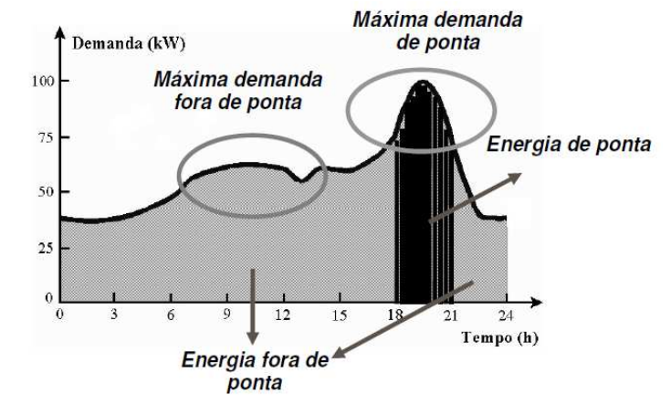
\includegraphics[width=.9\textwidth]{Figuras/ponta.png}
            \vspace*{\fill} 
            \begin{quote} 
            \centering 
            Fonte: \cite{procel}
            \end{quote}
            \vspace*{\fill}
			\label{fig:instres}
\end{center}
\end{figure}

Observando o funcionamento de uma instalação elétrica residencial, comercial
ou industrial, pode-se constatar que a potência elétrica consumida é variável a
cada instante. Isto ocorre porque nem todas as cargas instaladas estão todas em
funcionamento simultâneo. A potência total solicitada pela instalação da rede a
cada instante será, portanto, função das cargas em operação e da potência elé-
trica absorvida por cada uma delas a cada instante. \cite{procel}.

\subsubsection{Consumidor grupo A}

São os consumidores de alta tensão (tensão maior ou igual a 2.300 volts). \cite{procel}.

Para cargas com potência superior a 75kW é inconveniente para a concessionária realizar a alimentação de energia em baixa tensão, pois teria que construir subestações em via pública e instalar cabos de grande capacidade de corrente em propriedades particulares (empresas). \cite{procel}.

Define-se uma subestação como um conjunto de aparelhos e equipamentos destinados a modificar as características da energia elétrica (tensão e corrente), permitindo a sua distribuição aos pontos de consumo em níveis adequados de utilização. \cite{procel}.

Subestação do consumidor é aquela construída em propriedade particular suprida através de alimentadores de distribuição primários originados da concessionária. A partir da subestação a concessionária fará o fornecimento em tensão primária de 15 ou 25 kV. \cite{procel}.

Os consumidores do grupo A (média tensão = 2,3 kV até 69 kV) são classificados em:

\begin{itemize}
    \item A3 - 69 kV
    \item A3a -30 kV a 44 kV – normal 34,5kV
    \item A4 - 2,3 kV a 25 kV – normal 13,8kV
    \item AS - sistemas subterrâneos
\end{itemize}

\subsection{ESTRUTURA TARIFÁRIA}

\subsubsection{O horário de ponta}

\paragraph{test}

\hspace*{0.8cm}O  horário  de  ponta  é  o  período  de  três  horas  consecutivas  exceto  sábados, domingos e feriados nacionais no qual o consumo de energia elétrica está em seu ápice. 
    Nesse  período  a  tarifa  praticada  pela  concessionária  de  energia  aumenta consideravelmente,  pois  há  uma  elevação  do  consumo  em  nível  nacional, sobrecarregando os sistemas de geração, transmissão e distribuição. Esse período de três horas  é  definido  pela  concessionária  em  função  das  características  de  seu  sistema elétrico,  sendo  os  valores  máximos  atingidos  entre  as  17  e  22  horas. \cite{costa}

\begin{figure}[!htb]
\begin{center}
			\caption{Características da curva de carga diária de um consumidor genérico.}

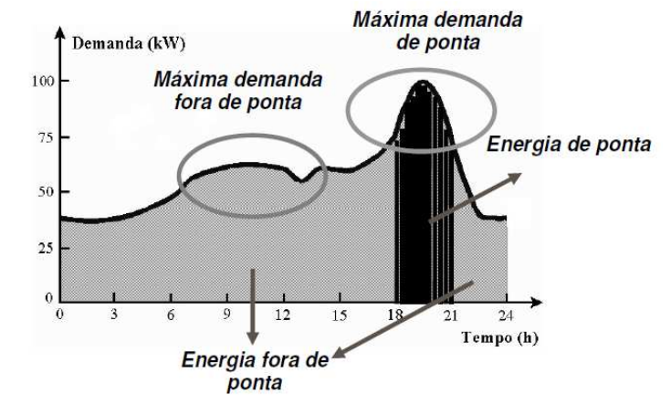
\includegraphics[width=.9\textwidth]{Figuras/ponta.png}
            \vspace*{\fill} 
            \begin{quote} 
            \centering 
            Fonte: \cite{procel}
            \end{quote}
            \vspace*{\fill}
			\label{fig:ponta}
\end{center}
\end{figure}

Gerar  energia  para  consumo  no  horário  de  ponta  tem  o  inconveniente  da  necessidade  de trocar a  fonte  supridora  duas  vezes  por  dia,  no início e ao término  do  período,  nos  dias  úteis.  Embora  a  transferência  de  carga  possa  ser  feita  rapidamente,  haverá interrupção do suprimento de energia, o que poderá ser inaceitável para algumas  atividades que não estejam protegidas por fontes de energia segura. Para solucionar este inconveniente,  pode-se  dotar  o(s)  grupo(s)  gerador(es)  com  sistemas  de  transferência  em transição fechada, sem interrupção e passagem da carga de uma para outra fonte em  rampa suave. Entretanto, para isso é necessário operar instantaneamente na condição de  paralelismo com a rede da concessionária. \cite{costa}